% Supporting Information for the preprint (main.tex). Build this file first: main.tex reads si.aux (xr) for the
% S-numbers of the figures, tables and sections cited from the main text.
\documentclass[journal=jacsat,manuscript=suppinfo]{achemso}

\usepackage[version=4]{mhchem}
\usepackage{amsmath}
\usepackage{amssymb}
\usepackage{siunitx}
\usepackage{booktabs}
\usepackage{longtable}
\usepackage{tabularx}
\graphicspath{{figs/}{../../figures/}}
\SectionNumbersOn
\renewcommand{\thefigure}{S\arabic{figure}}
\renewcommand{\thetable}{S\arabic{table}}
\renewcommand{\thesection}{S\arabic{section}}

\author{Chan Young Joe}
\affiliation{Independent Researcher, Incheon, Republic of Korea}
\email{ccy5123ccy@gmail.com}
\title{Silent but deadly? Physics says seldom, memory says mostly}

\begin{document}
\maketitle

\begin{figure}
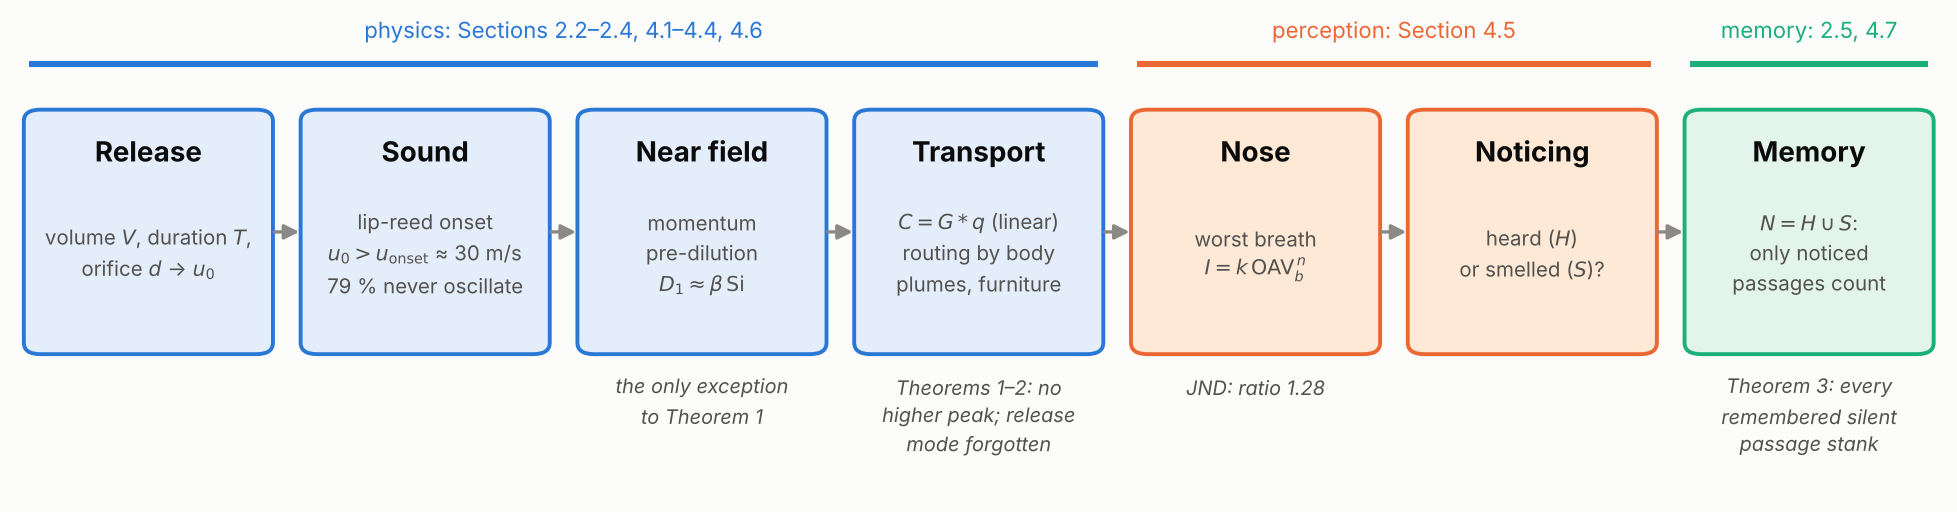
\includegraphics[width=\textwidth]{fig2_chain.png}
\caption{From release to memory: the quantity each stage passes on, and where Theorems 1--3 apply.}
\label{fig:chain}
\end{figure}

\section{CFD validation}
\label{sec:si-validation}
\begin{itemize}
  \item \emph{Free round jet} (axisymmetric, $\mathrm{Re} = 6700$, three meshes). The velocity-decay constant is 5.0 and
  the scalar constant $K_c = 4.3$--4.6, with a grid uncertainty of at most 3.7\%. The $k$--$\omega$ SST model spreads
  round jets about 25\% too fast, which over-dilutes audible releases by about 15\% and so favours the silent release.
  \item \emph{Convective boundary layer} of a simplified seated manikin with skin at 33\,\textdegree C, compared with
  thermal-manikin data \cite{licina2014}. The face-front peak velocity is 40--56\% too high at room temperatures of
  20--26\,\textdegree C; its change with room temperature is reproduced ($-27\%$ against $-33\%$ measured). The fast
  boundary layer shortens travel times to the releaser's own nose by about 30\%, and the analytic model stretches the
  CFD travel times by a factor of 1.4 to correct for it.
\end{itemize}

\begin{figure}
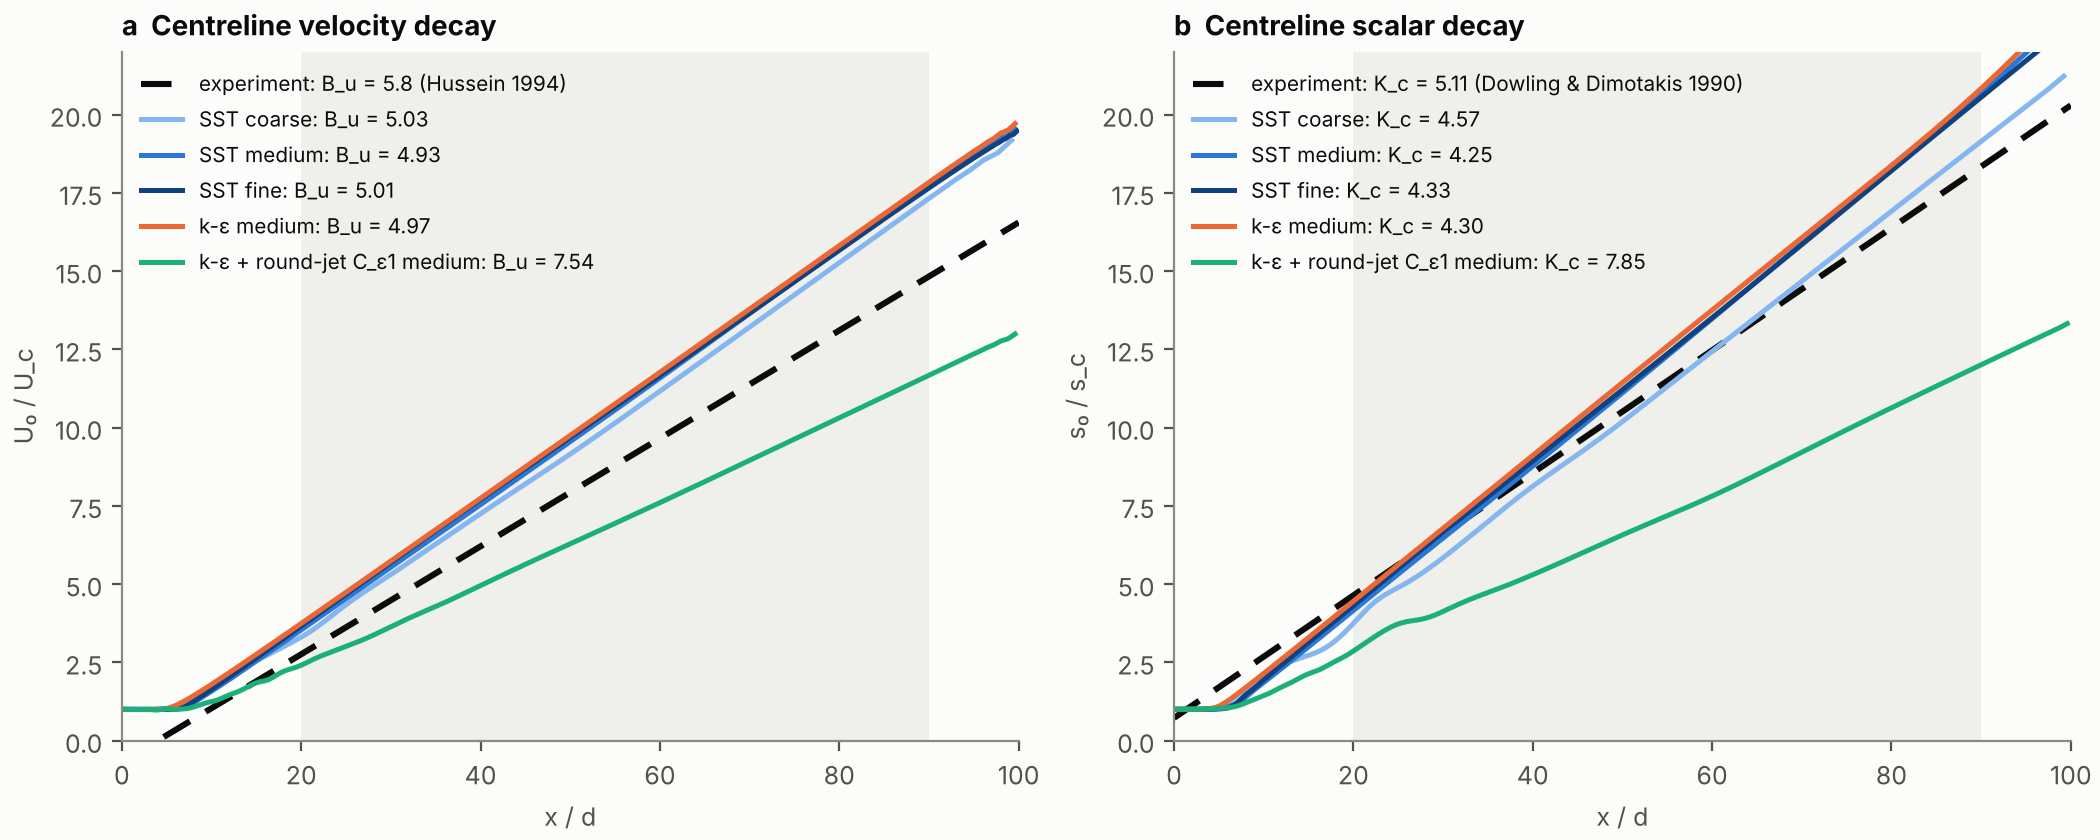
\includegraphics[width=\textwidth]{fig4_jet_validation.png}\\[4pt]
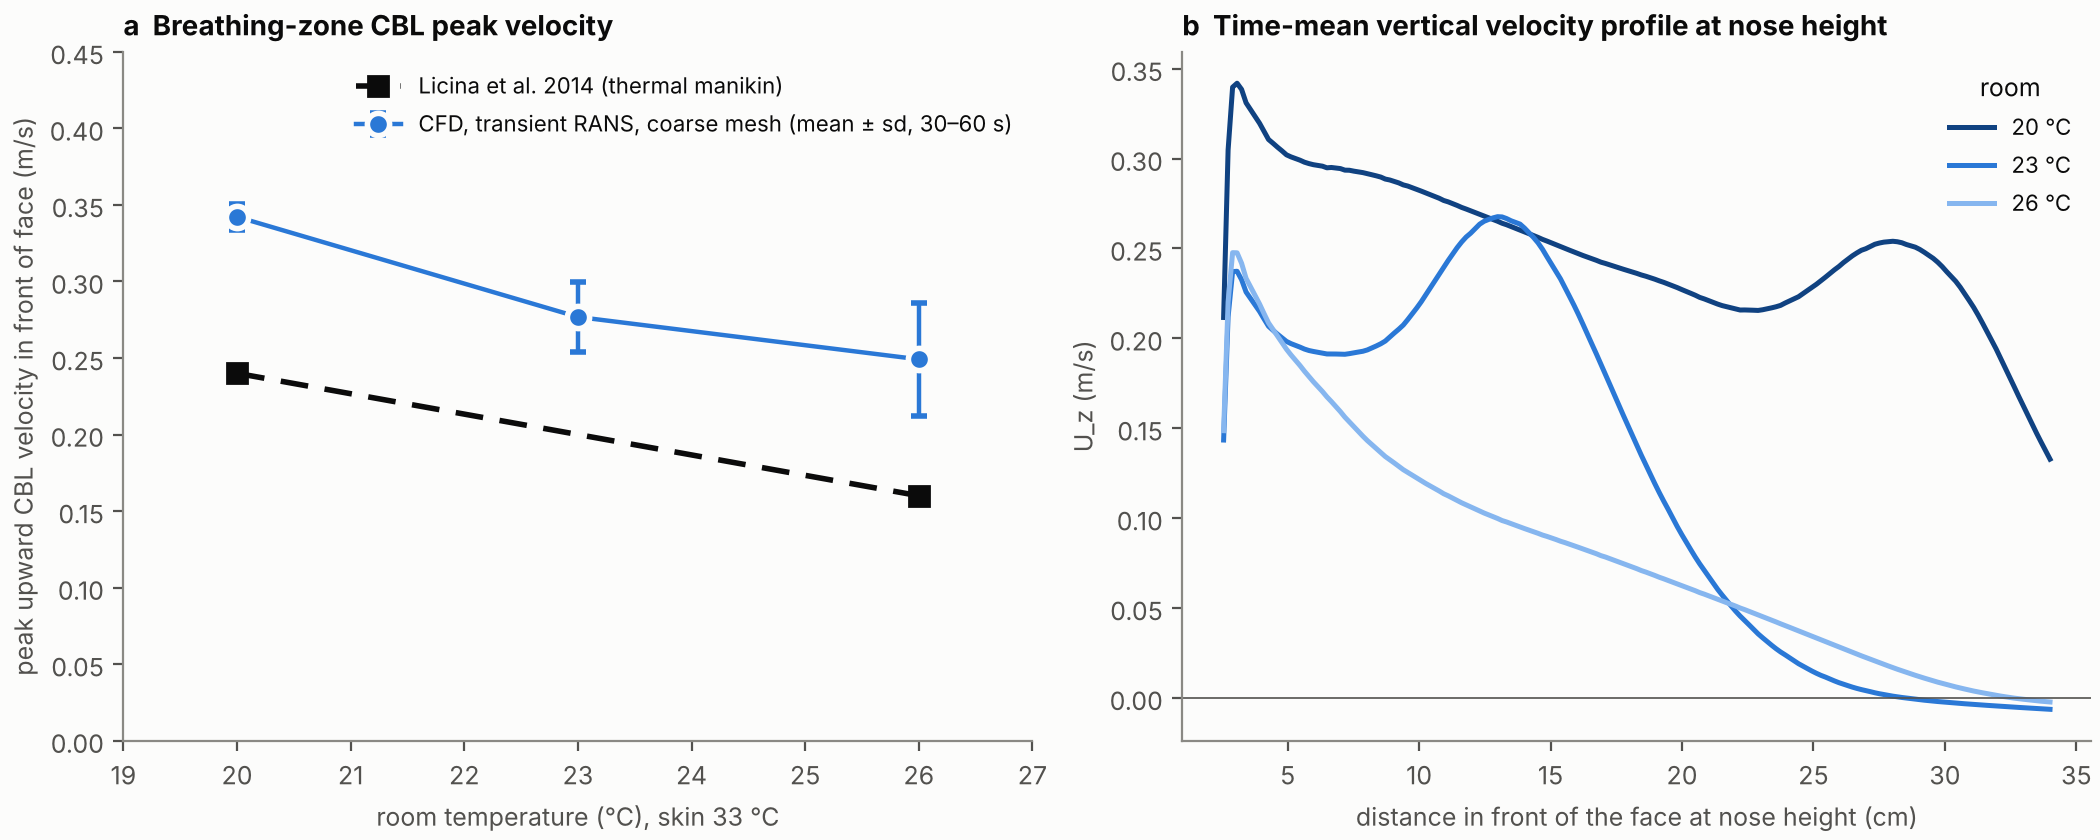
\includegraphics[width=\textwidth]{fig4_cbl_validation.png}
\caption{Validation. Top: free round jet at $\mathrm{Re} = 6700$ on three meshes (centreline velocity and scalar decay,
spreading). Bottom: face-front convective boundary layer of the seated manikin against thermal-manikin data
\cite{licina2014} at 20--26\,\textdegree C, and time-mean vertical velocity profiles at nose height.}
\label{fig:validation}
\end{figure}

\section{CFD scenes}
\label{sec:si-scenes}
All scenes use the solver of the main text, skin at 33\,\textdegree C and walls at 23\,\textdegree C. Each is first run
without a release until the body plumes have developed (30\,s; 90\,s with ventilation). From that flow field the same
92\,mL is released behind the releaser's buttocks, pointing down and back, as an inlet that matches the release's
volume flow and momentum: silent, 2\,s through 8\,mm ($u_0 = 0.9$\,m\,s$^{-1}$); audible, 0.5\,s through 2.4\,mm
(41\,m\,s$^{-1}$). The odorant is a passive scalar, sampled 2.5\,cm in front of each nose, over 5\,cm discs at nose
height (breathing zone) and over sinusoidal breathing cycles; the worst breath is the most concentrated single
inhalation.

\begin{itemize}
  \item \emph{Sofa.} A 3.2 $\times$ 3.2 $\times$ 2.6\,m living room with a 0.5\,m ceiling vent for pressure relief
  (size and position assumed). Two seated manikins sit 0.6\,m apart on a two-seat sofa whose base is solid to the
  floor. Mesh 0.72 million cells, refined to 5\,mm at the release and 2.5\,mm on the inlet face. Runs of 30\,s, the
  upright one extended to 120\,s. Two variants rotate the releaser's upper body about the hip: reclined by
  4.5\,\textdegree, so that the back closes onto the backrest, and leaning forward by 10\,\textdegree, so that the gap
  behind the back opens.
  \item \emph{Elevator.} The car of a 630\,kg, eight-person elevator, 1.10\,m wide, 1.40\,m deep and 2.10\,m high (a
  manufacturer's standard car, within the maximum area of 1.66\,m$^2$ allowed for that load). Four standing manikins
  (nose at 1.59\,m) stand in a $2 \times 2$ grid facing the door; the fan is off, and a 0.2\,m ceiling opening relieves
  pressure (size assumed). Mesh 0.91 million cells. Runs of 60\,s with the release behind a front-row or a back-row
  occupant; mirror symmetry gives the other two positions.
  \item \emph{Standing pair.} The sofa room without the sofa, with two standing manikins face to face, noses 1.0\,m
  apart and 0.8\,m of open floor behind each back. Still air and office ventilation share one mesh of 0.43 million
  cells. Ventilation is one square ceiling diffuser above the pair supplying 21.2\,L\,s$^{-1}$, i.e.\ 2.9 air changes
  per hour (EN 16798-1 Category II for two people in a low-polluting 10\,m$^2$ room: 7\,L\,s$^{-1}$ per person plus
  0.7\,L\,s$^{-1}$\,m$^{-2}$ \cite{olesen2024}). The air leaves the diffuser along the ceiling at an assumed
  1.5\,m\,s$^{-1}$, at room temperature, and exits through a ceiling grille. Runs of 60\,s.
\end{itemize}

\section{Sofa}
\label{sec:si-sofa}
\emph{Silent release.} The silent release stays in the convective boundary layer of the releaser's back. It rises in
the gap between back and backrest, over the head and to the ceiling. Within 30\,s its breathing-zone OAV is at most
$10^{-10}$ at both noses, while within 25\,cm of the releaser's head it reaches 6\,000.

\emph{Audible release.} The audible jet hits the corner between seat and backrest, spreads sideways along the gap and
rises up both backs as a wider, more dilute sheet; part of it curls around the heads. It reaches the neighbour's head
region within 6\,s and both breathing zones at OAV 0.2--0.6.

\emph{Reclined by 4.5\,\textdegree.} With the back closed onto the backrest, the silent release leaves the seat-level
wedge sideways and still rises behind the head; no breathing zone receives more than $10^{-10}$. The audible jet wraps
around the releaser's face and exceeds threshold at their own nose (OAV 2--4).

\emph{Leaning forward by 10\,\textdegree.} With the gap behind the back open, both releases rise behind the head, and
the releaser's nose, 13\,cm further forward, receives neither (breathing-zone OAV $\le 10^{-5}$). The silent cloud
reaches the region within 25\,cm of the neighbour's head as strongly as the audible one (OAV 580 against 450) but not
the neighbour's breathing zone ($10^{-4}$); the audible jet reaches it at OAV 2.6.

\emph{120\,s.} Both clouds reach the ceiling, return through the room and arrive at both noses from about 45\,s. After
about 70\,s the silent and audible traces at the neighbour are indistinguishable (worst breath 0.39 for both). At the
releaser's own nose the mixed silent cloud is 1.5--2 times higher and touches the trained-panel threshold for about a
second near 100\,s. These levels are 10--23 times below the thresholds of untrained observers.

\begin{table}
\caption{Sofa: peak breathing-zone OAV within 30\,s of the release (mean flow).}
\label{tab:sofa}
\begin{tabular}{llcc}
\toprule
nose & posture & silent & audible \\
\midrule
releaser & upright & $5\times10^{-11}$ & 0.46 \\
releaser & reclined 4.5\,\textdegree & $9\times10^{-11}$ & 3.3 \\
releaser & forward 10\,\textdegree & $3\times10^{-7}$ & $1.5\times10^{-5}$ \\
neighbour & upright & $3\times10^{-14}$ & 0.63 \\
neighbour & reclined 4.5\,\textdegree & $3\times10^{-15}$ & 0.19 \\
neighbour & forward 10\,\textdegree & $1\times10^{-4}$ & 2.6 \\
\bottomrule
\end{tabular}
\end{table}

\begin{figure}
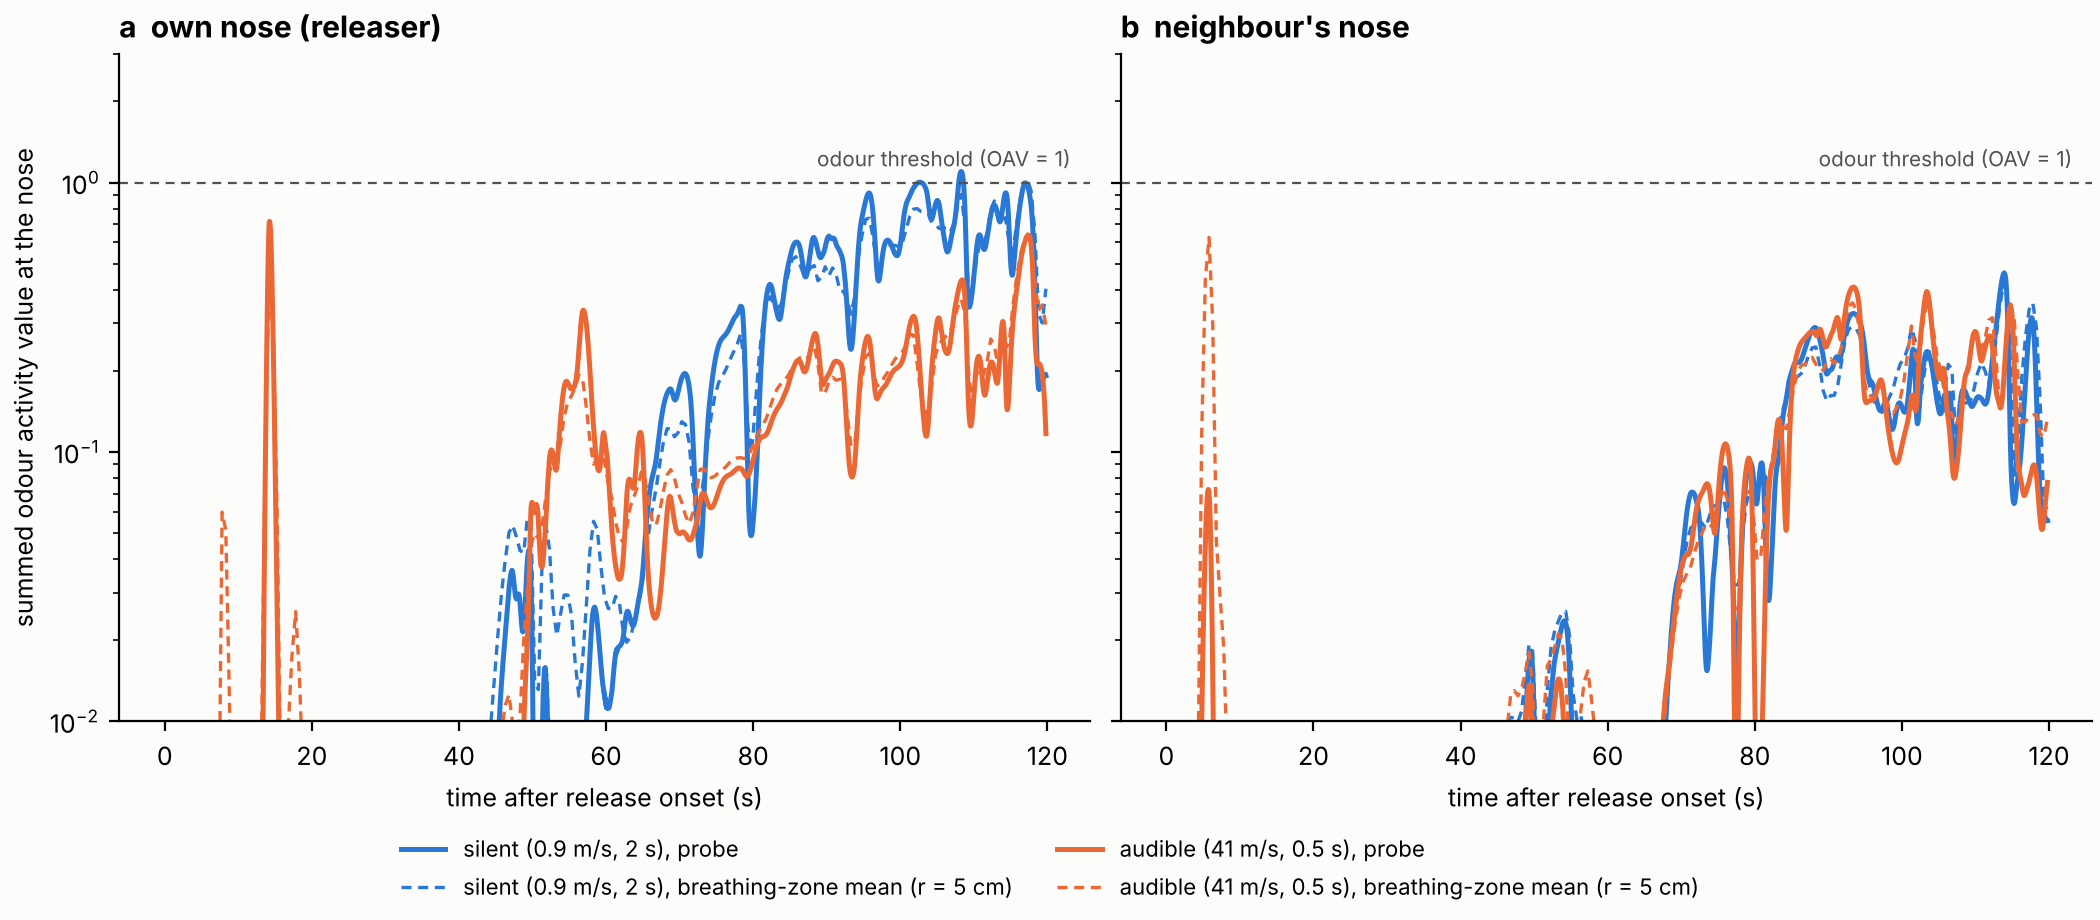
\includegraphics[width=\textwidth]{fig5_sofa_duet_noses.png}
\caption{Sofa, upright: OAV at the releaser's and the neighbour's nose over 120\,s for the same 92\,mL released
silently or audibly. Solid: 2.5\,cm in front of the nose; dashed: mean over a 5\,cm breathing-zone disc. The
horizontal line is the trained-panel odour threshold.}
\label{fig:sofa-noses}
\end{figure}

\begin{figure}
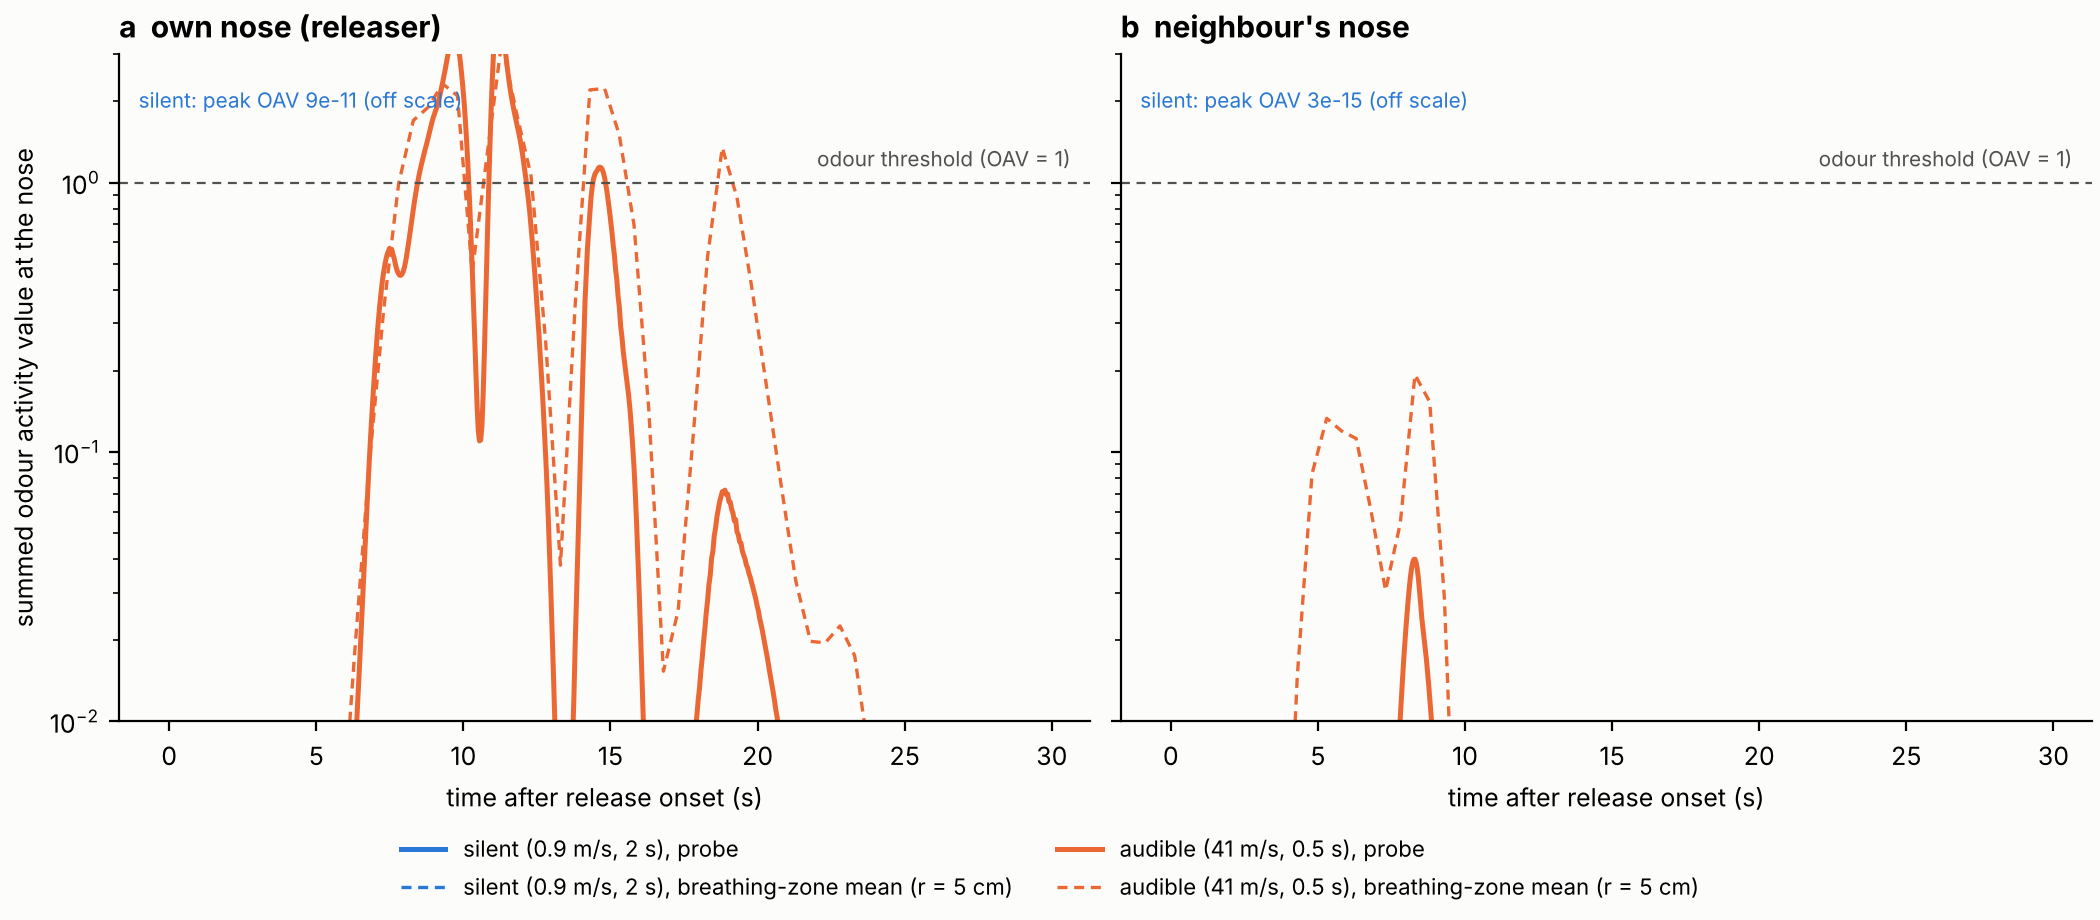
\includegraphics[width=0.49\textwidth]{figS_sofa_rec4.5_noses.png}\hfill
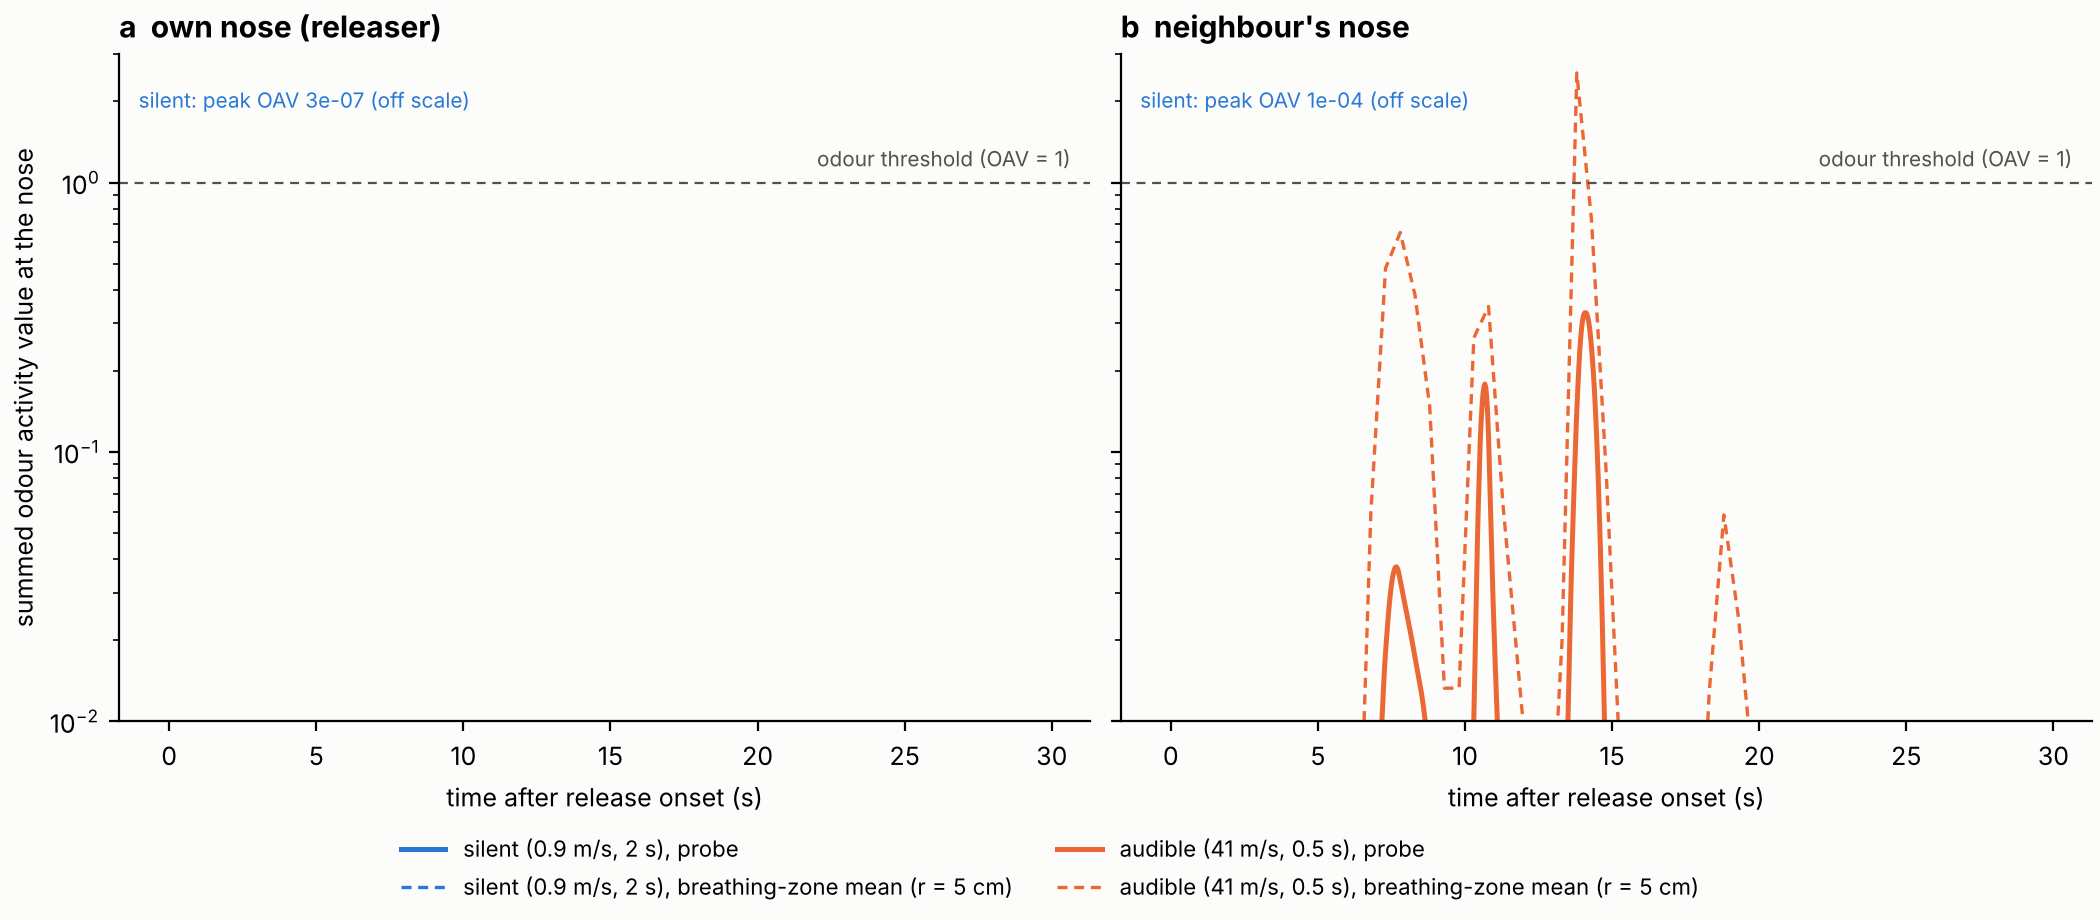
\includegraphics[width=0.49\textwidth]{figS_sofa_rec-10_noses.png}\\[4pt]
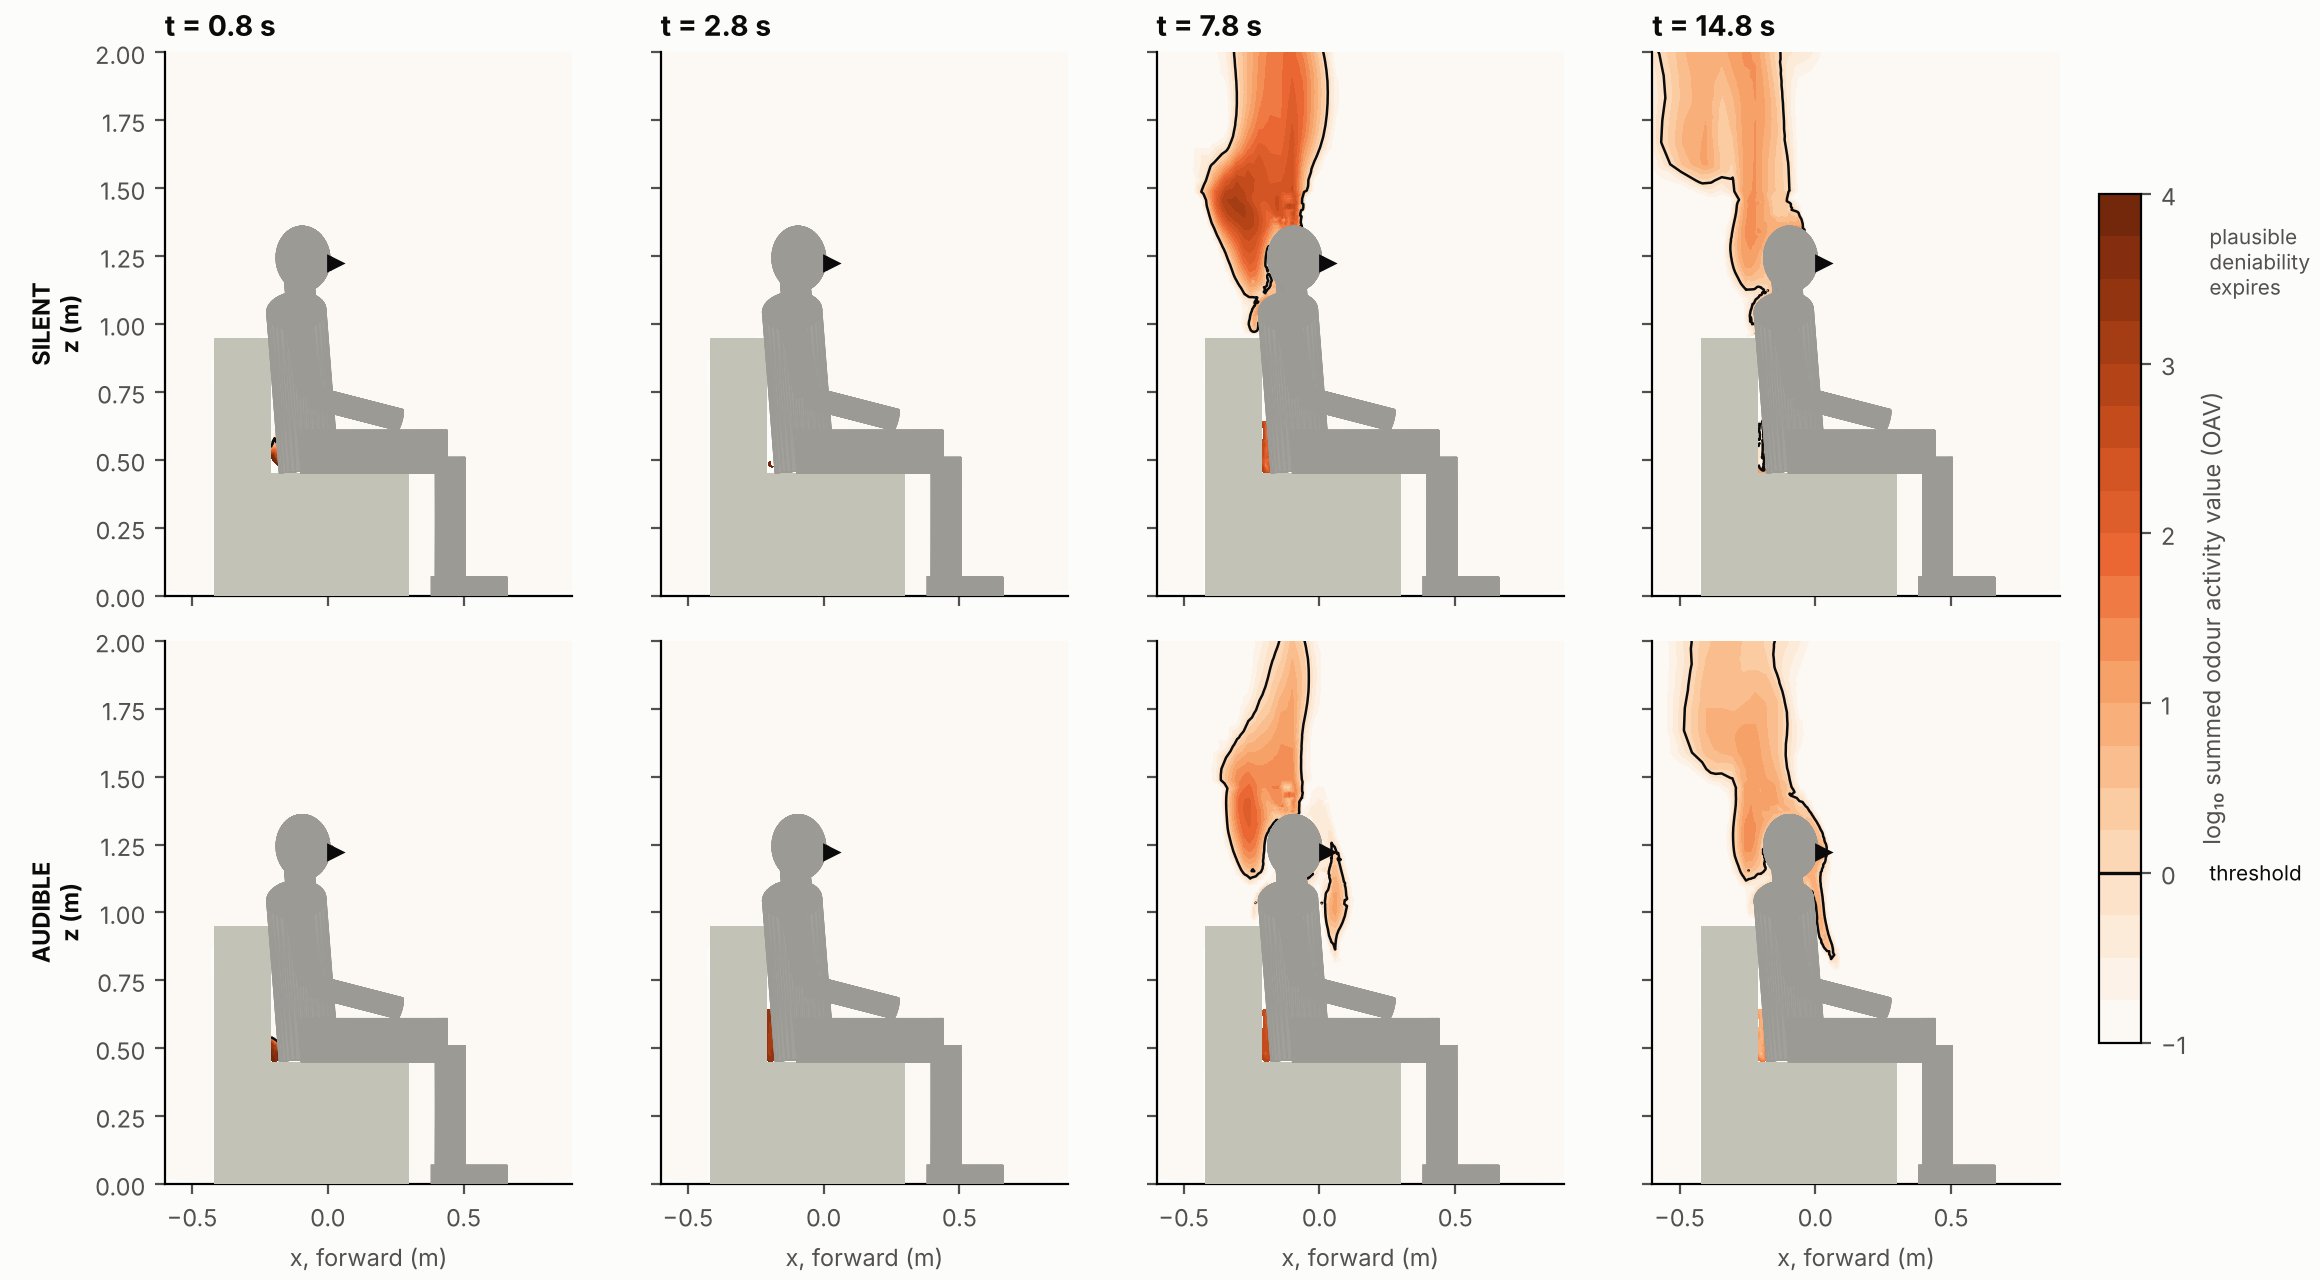
\includegraphics[width=0.49\textwidth]{figS_sofa_rec4.5_planes.png}\hfill
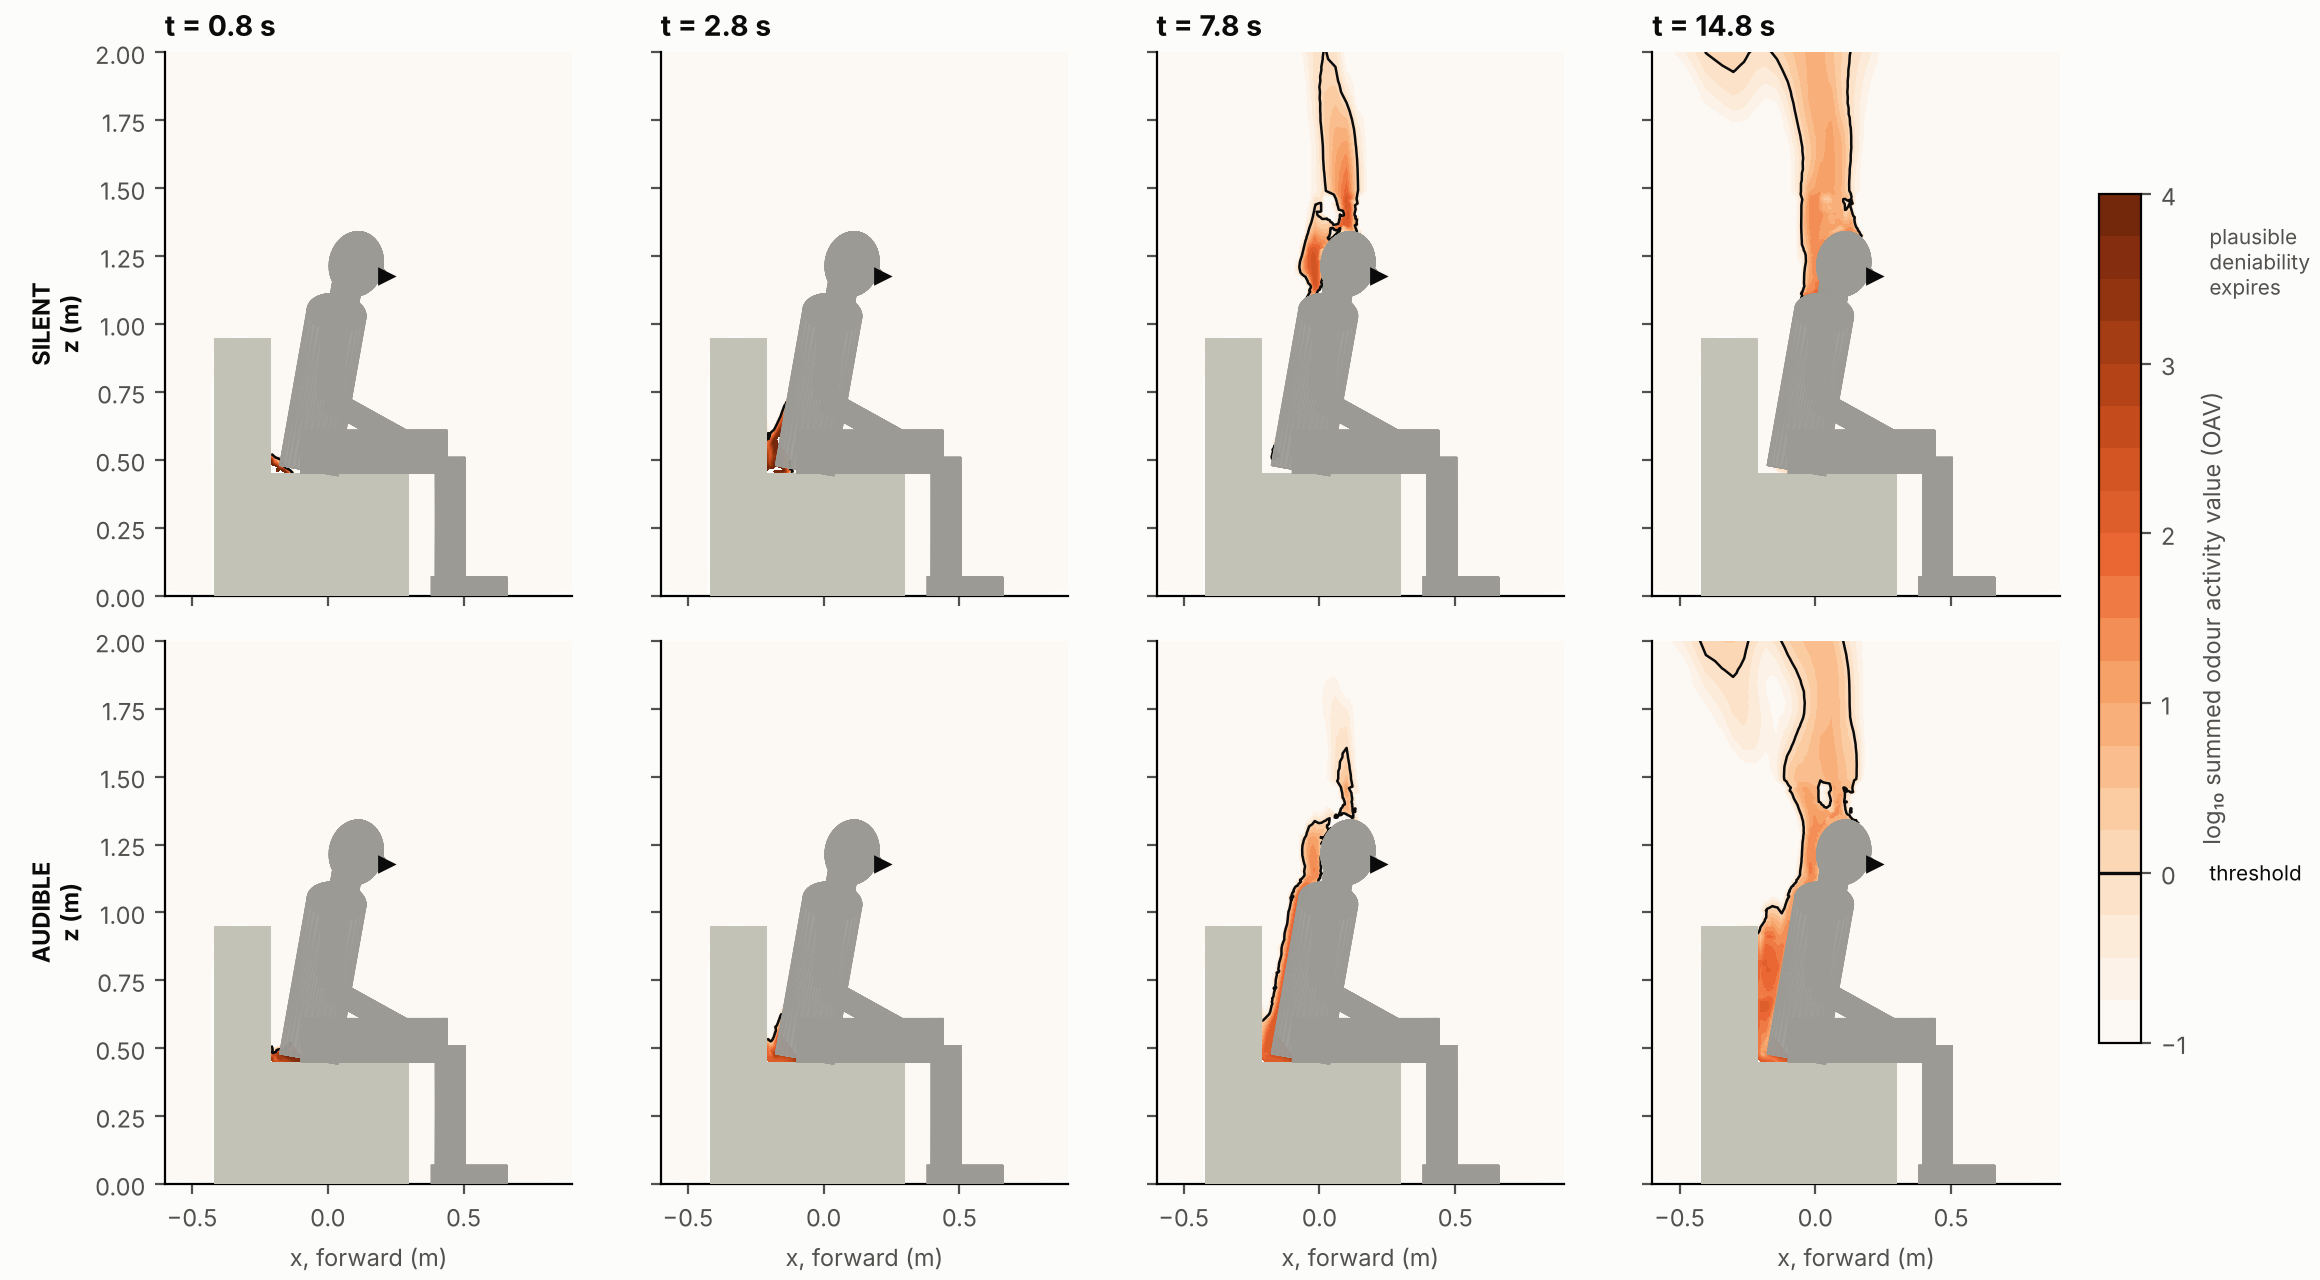
\includegraphics[width=0.49\textwidth]{figS_sofa_rec-10_planes.png}
\caption{Sofa, releaser reclined by 4.5\,\textdegree\ (left) or leaning forward by 10\,\textdegree\ (right), 30\,s.
Top: OAV at both noses, as in Figure~\ref{fig:sofa-noses}. Bottom: log$_{10}$ OAV in the releaser's mid-sagittal
plane, silent (upper rows) and audible (lower rows).}
\label{fig:sofa-postures}
\end{figure}

\section{Elevator}
\label{sec:si-elevator}
A silent release follows the releaser's own back plume, so what stands behind the releaser decides where it goes.
\begin{itemize}
  \item With a person behind (front-row releaser), it rises in the 0.2\,m gap between the releaser's back and that
  person's face, into their breathing zone. The silent release is stronger at every nose ($R = 1.4$--$4.3$), most of
  all for the person behind (OAV 27).
  \item With the car wall behind (back-row releaser), it rises between back and wall and reaches the front row only
  below threshold. The audible jet hits the floor, is lifted by all four body plumes, and is stronger at every nose
  ($R = 0.20$--$0.55$).
\end{itemize}
With a front-row releaser the person behind reaches the trained-panel threshold first (8.8\,s), before the releaser
(17.6\,s); with a back-row releaser the releaser is first. Whoever smells it first is therefore the releaser in half
of the positions, for both modes.

\emph{Identifying the releaser.} Each occupant other than the releaser reacts with the detection probability of the
main text's observer models, independently. Onlookers see only who reacted and infer the releaser with a uniform
prior, for a releaser who never reacts and one who reacts like the others. With distracted occupants no one reacts in
87--92\% of passages, and the releaser is identified at 0.28--0.31; attentive occupants identify the releaser at
0.39--0.52 (chance 0.25). Silent and audible passages are identified about equally well by odour; the sound of an
audible passage, which also points to the releaser, is not modelled.

\begin{table}
\caption{Elevator: expected worst-breath OAV within 60\,s at each nose (trained-panel thresholds; mean flow), for a
front-row and a back-row releaser.}
\label{tab:elevator}
\begin{tabular}{llccc}
\toprule
releaser & nose & silent & audible & $R$ \\
\midrule
front row & releaser & 6.7 & 1.9 & 3.4 \\
 & beside & 3.6 & 0.8 & 4.3 \\
 & behind & 27 & 20 & 1.4 \\
 & diagonal & 7.6 & 2.7 & 2.9 \\
back row & releaser & 4.5 & 23 & 0.20 \\
 & beside & 2.3 & 5.9 & 0.39 \\
 & in front & 0.57 & 2.8 & 0.20 \\
 & diagonal & 0.41 & 0.74 & 0.55 \\
\bottomrule
\end{tabular}
\end{table}

\begin{figure}
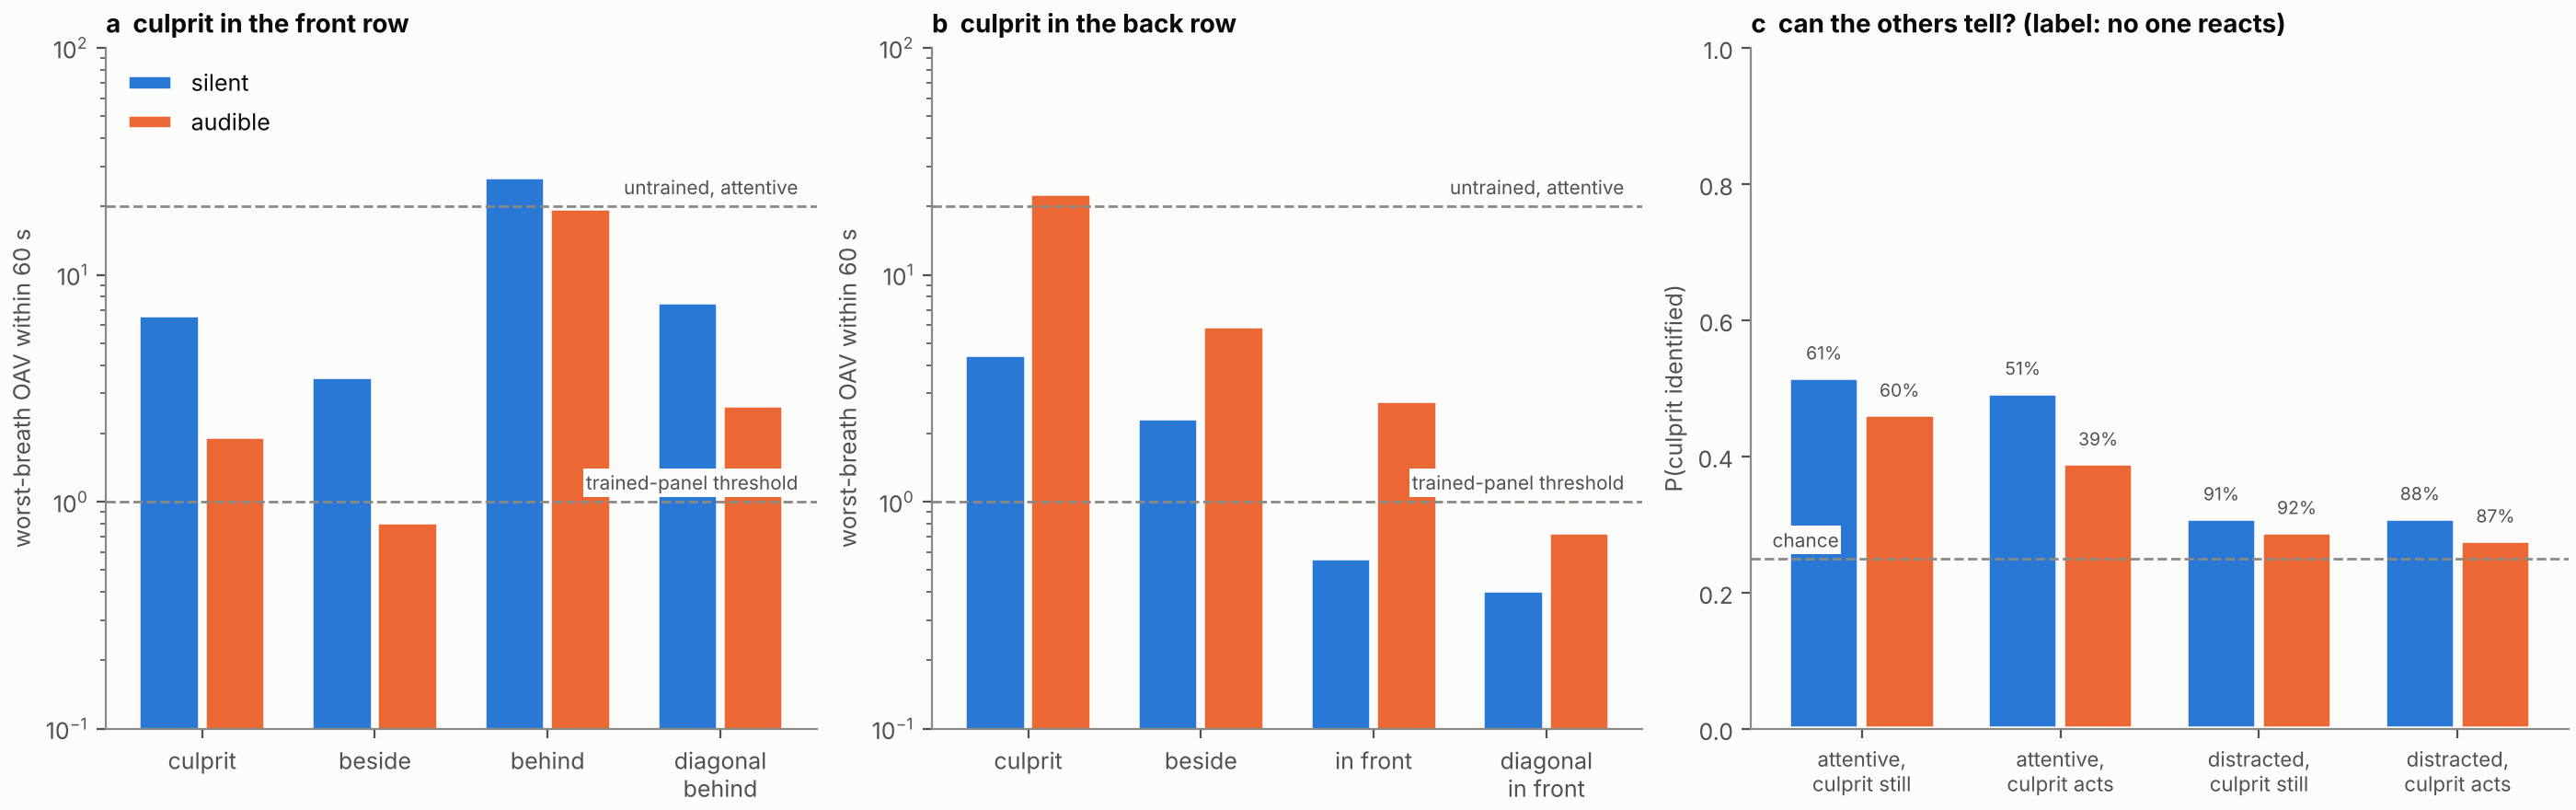
\includegraphics[width=\textwidth]{fig15_elevator.png}
\caption{Elevator: four standing occupants in a closed 630\,kg car, fan off, same 92\,mL. (a, b) Expected
worst-breath OAV within 60\,s at each nose for a front-row and a back-row releaser; dashed lines mark the
trained-panel threshold and the attentive population threshold. (c) Probability that the others identify the
releaser from who reacted, for attentive and distracted onlookers and a releaser who stays still or reacts along;
labels give the probability that no one reacts. The dashed line is chance.}
\label{fig:elevator}
\end{figure}

\section{Standing pair}
\label{sec:si-standing}
Results pending (simulations running).

\section{Breath sampling}
\label{sec:si-breath}
An audible puff reaches the neighbour after a median of 16\,s and passes with a time scale of about 3.8\,s
(10--90\%: 1.4--12\,s). Without a warning, the breathing phase barely matters: for a median passage the worst breath
captures 81--99\% of the peak. A listener warned by the sound needs about 23\,s of breath-hold for an even chance of
missing the puff (worst breath below 10\% of the peak); 33\,s, the typical maximum at end-expiration, gives 68\%.

\begin{figure}
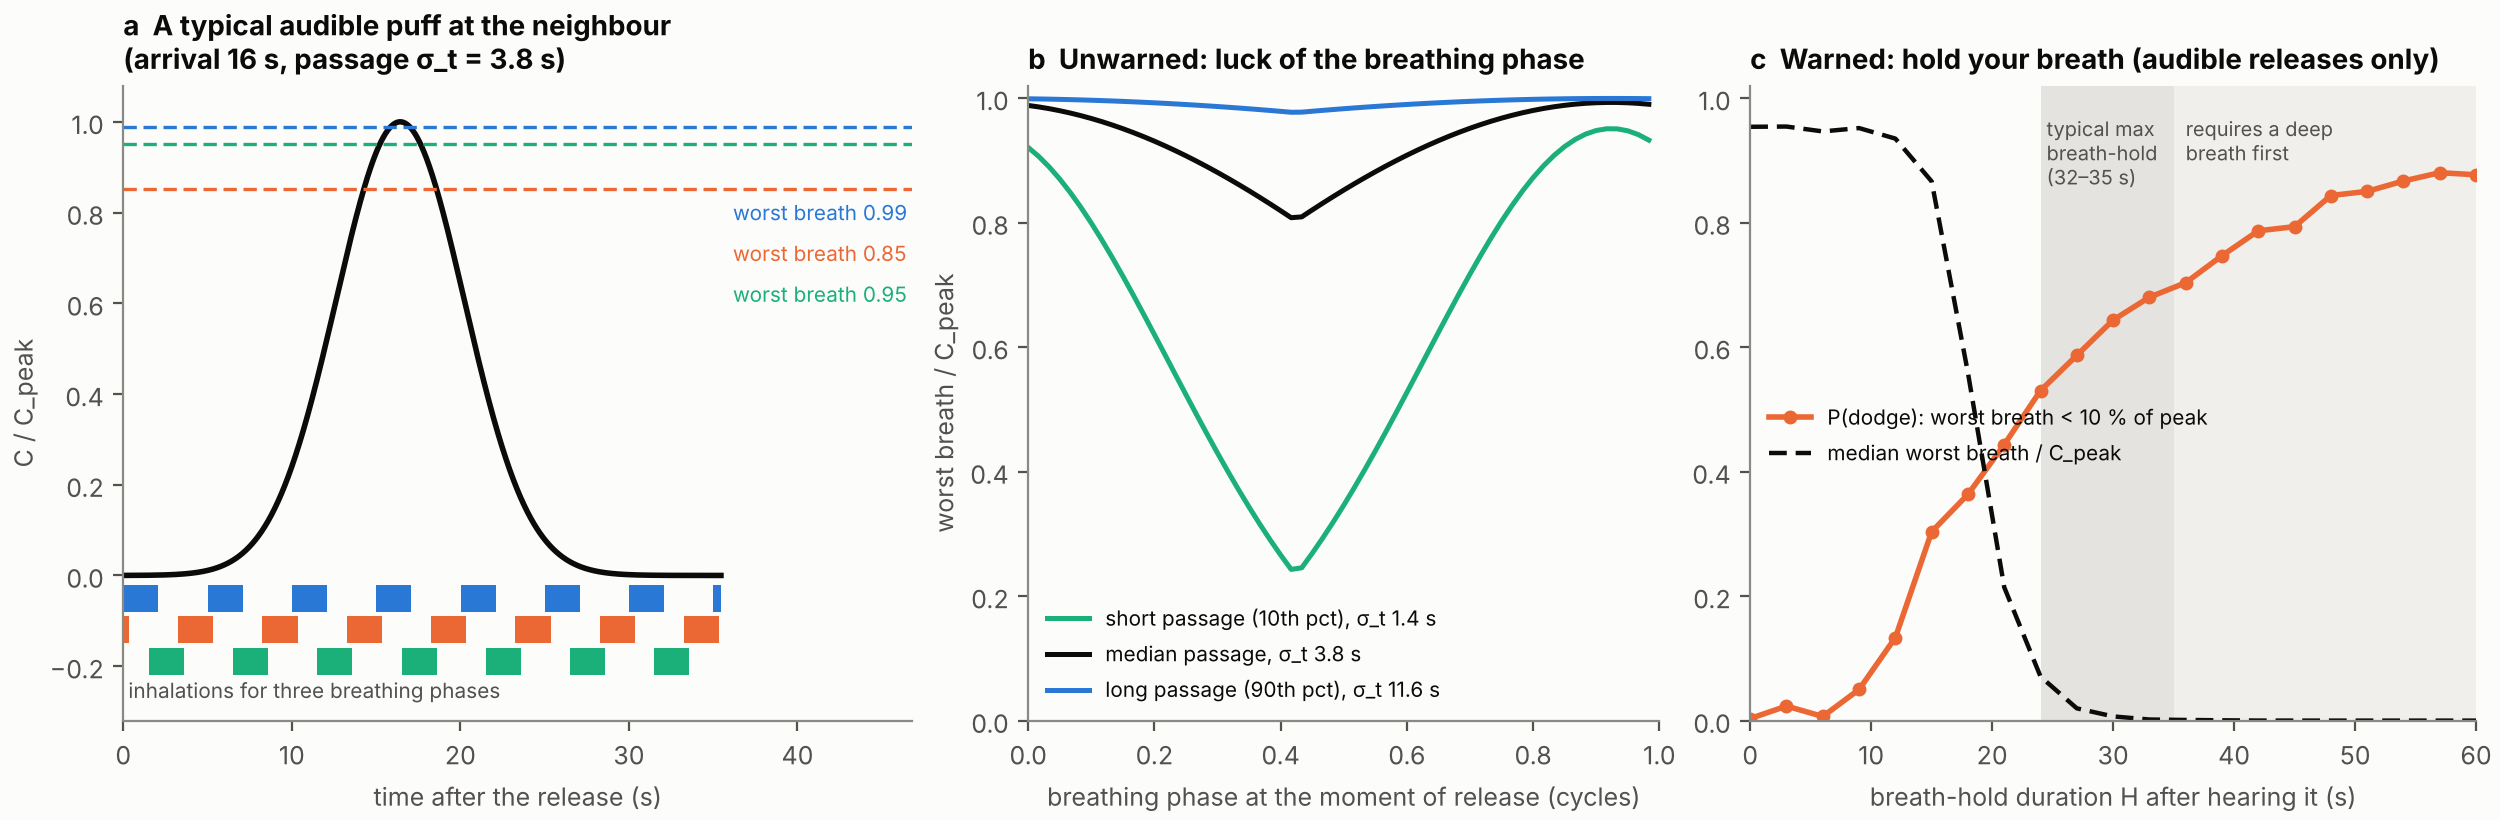
\includegraphics[width=\textwidth]{fig7_breath_hold.png}
\caption{Breath sampling at the neighbour's nose for audible releases. (a) A typical puff (arrival 16\,s, passage
time scale 3.8\,s) and the inhalations of three breathing phases, with the worst breath of each. (b) Without warning:
worst breath relative to the peak against the breathing phase at release, for short, median and long passages. (c)
Warned: probability of missing the puff (worst breath below 10\% of the peak) and median worst breath, against the
breath-hold duration after hearing the release (0.5\,s reaction latency).}
\label{fig:breath}
\end{figure}

\section{Cross-cultural survey}
\label{sec:si-culture}
We searched dictionaries, proverb collections and etymological handbooks in 32 languages or historical stages for a
dedicated word for a silent passage and for an explicit claim that it smells worse, and checked every entry used
against a retrieved source. Each language is graded by its strongest evidence: A, an explicit saying (traditional,
or in media or film only); B, a dedicated word defined by its smell; C, a dedicated word without a smell claim; D,
nothing found. The silent/loud distinction is lexicalised in at least five language families. The explicit claim is
traditional only in Chinese and English, and smell-defined silent words arose independently at least four times
within Indo-European. The survey records whether the belief is documented in a language, not how many speakers hold
it.

\begin{figure}
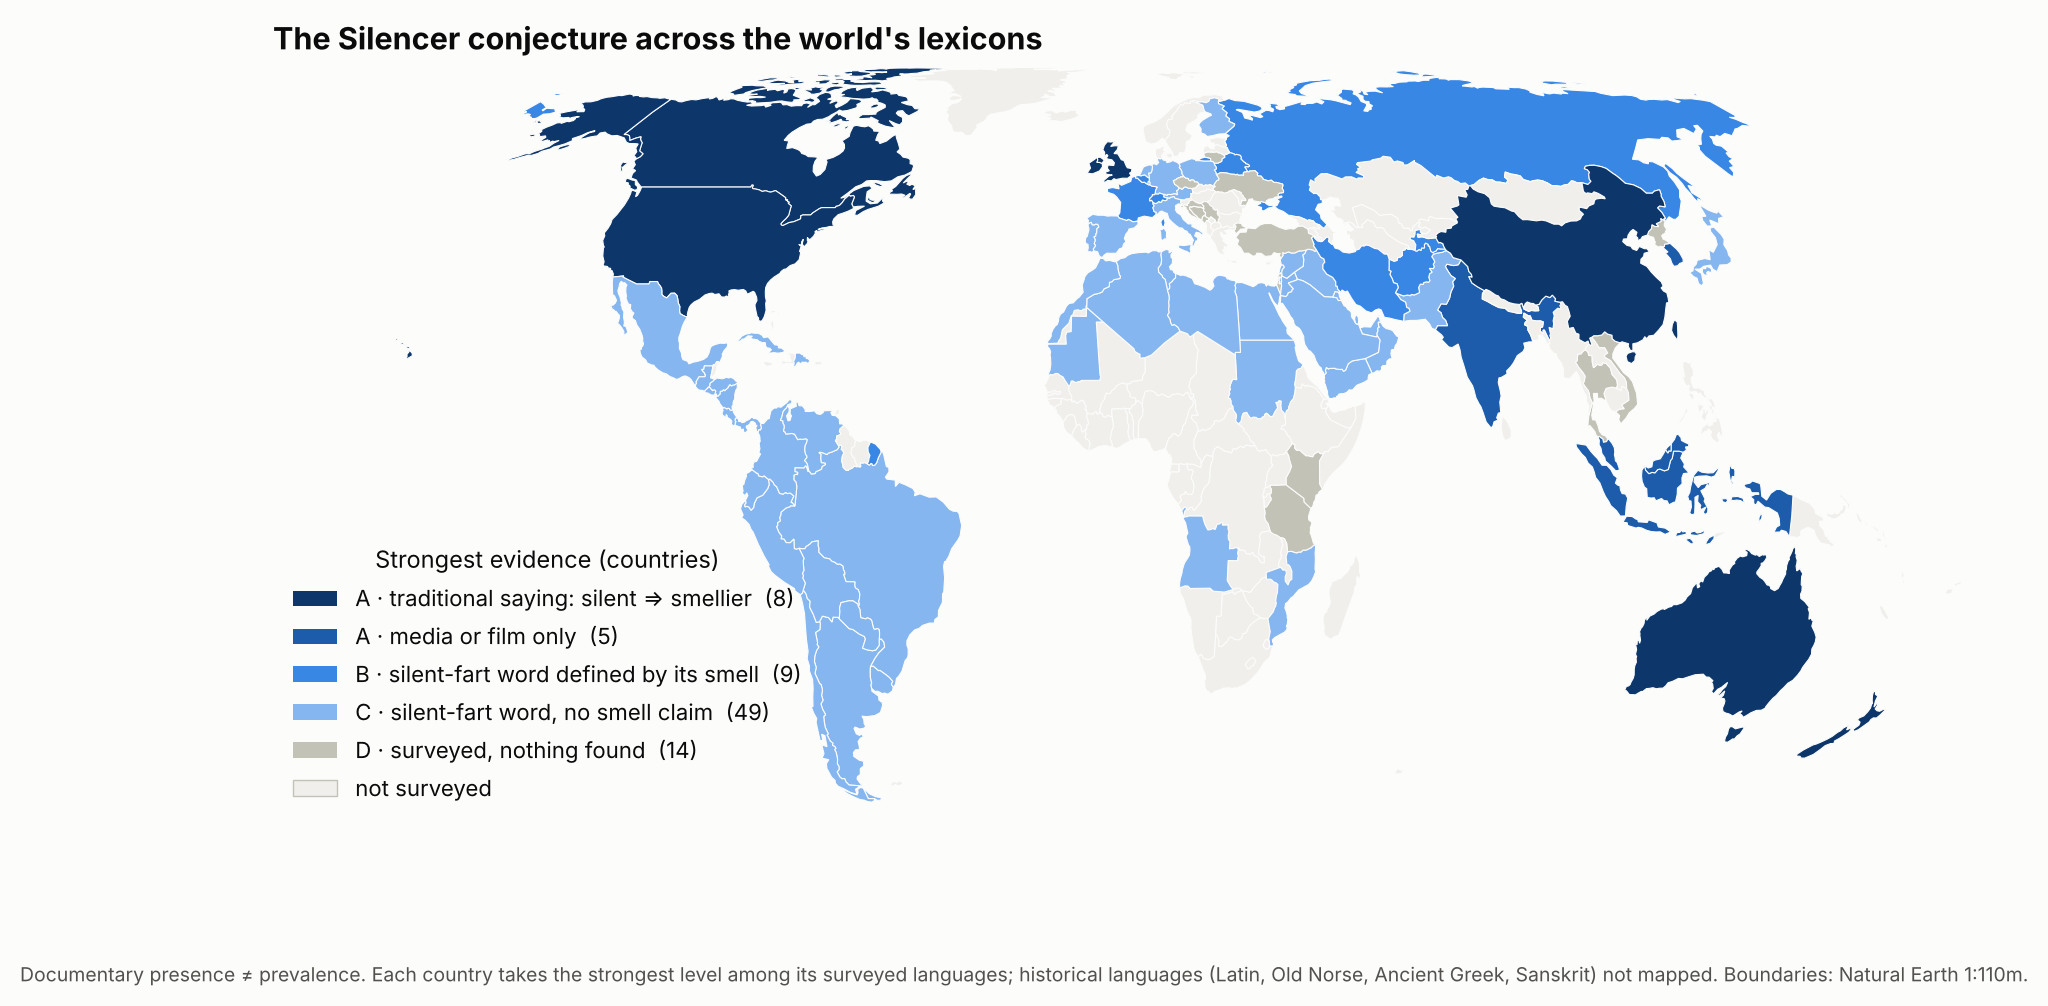
\includegraphics[width=\textwidth]{fig12_culture_map.png}
\caption{The belief across languages, by evidence level. Each country takes the strongest level among its surveyed
languages. A: an explicit saying that silent passages smell worse (traditional, or in media or film only); B: a
dedicated word for a silent passage defined by its smell; C: a dedicated word with no smell claim; D: surveyed,
nothing found.}
\label{fig:culture}
\end{figure}

\section{Code and data}
\label{sec:si-data}
The archive contains the code, inputs and outputs of every result; Table~\ref{tab:data} lists where each comes from.

\begin{table}
\caption{Source files of the results in the archive.}
\label{tab:data}
\small
\begin{tabularx}{\textwidth}{lX}
\toprule
result & files \\
\midrule
parameters (Table~\ref{tab:params}) & \texttt{params/params.yaml} \\
odorant shares, buoyancy, losses & \texttt{chem/odorants.py}, \texttt{chem/buoyancy.py}, \texttt{chem/reactivity.py}, \texttt{chem/chem\_report.md} \\
acoustics & \texttt{acoustics/regime.py}, \texttt{acoustics/run\_m2.py}, \texttt{acoustics/m2\_report.md} \\
analytic dispersion model & \texttt{gate0/model.py}, \texttt{gate0/run\_gate0.py}, \texttt{gate0/gate0\_report.md} \\
uncertainty, regime map & \texttt{uq/run\_m7.py}, \texttt{uq/m7\_report.md} \\
passages as emitted in the scenes & \texttt{uq/routing\_headline.py}, \texttt{uq/routing\_headline.json}, \texttt{uq/fig\_routing.py} \\
CFD validation & \texttt{cfd/validation/jet}, \texttt{cfd/validation/cbl}, \texttt{cfd/validation/m3\_report.md} \\
sofa & \texttt{cfd/cases/sofa}, \texttt{cfd/cases/sofa/m4\_report.md} \\
elevator & \texttt{cfd/cases/elevator}, \texttt{cfd/cases/elevator/m5\_report.md} \\
standing pair & \texttt{cfd/cases/standing} \\
geometry & \texttt{cfd/geometry/manikin.py} \\
breath sampling, perception & \texttt{perception/model.py}, \texttt{perception/run\_m6.py}, \texttt{perception/m6\_report.md} \\
observer models, memory & \texttt{uq/observer\_ps.py}, \texttt{perception/selection.py}, \texttt{perception/run\_selection.py} \\
cross-cultural survey & \texttt{culture/cross\_cultural\_table.csv}, \texttt{culture/survey\_summary.md} \\
\bottomrule
\end{tabularx}
\end{table}

\section{Parameters}
\label{sec:si-params}
{\small\setlength{\tabcolsep}{4pt}
% Generated by make_params_table.py from params/params.yaml. Do not edit by hand.
\begin{longtable}{lllll}
\caption{Model parameters: nominal value, range sampled or tested, and status (VERIFIED, DERIVED, PARTIAL, ASSUMPTION). Sources and notes for every entry are in \texttt{params/params.yaml} of the code archive.}\label{tab:params}\\
\toprule
parameter & nominal & range & units & status \\
\midrule
\endhead
\multicolumn{5}{l}{\textit{Source}} \\
\texttt{T\_gas} & 310.15 & 309.85--310.65 & K & VERIFIED \\
\texttt{V\_passage} & $9.2\times10^{-5}$ & $1.7\times10^{-5}$--$3.75\times10^{-4}$ & m$^3$ & VERIFIED \\
\texttt{V\_daily} & $7.05\times10^{-4}$ & $4.76\times10^{-4}$--0.001491 & m$^3$\,d$^{-1}$ & VERIFIED \\
\texttt{n\_daily} & 10 & 1--20 & d$^{-1}$ & VERIFIED \\
\texttt{d\_orifice} & 0.004 & 0.001--0.015 & m & ASSUMPTION \\
\texttt{T\_release} & 1 & 0.3--5 & s & ASSUMPTION \\
\texttt{dp\_rectal} & 2000 & 500--4000 & Pa & ASSUMPTION \\
\texttt{p\_anal\_rest} & 8666 & 6133--12000 & Pa & VERIFIED \\
\texttt{g\_reduced} & 1.7 & -0.66--4.68 & m\,s$^{-2}$ & DERIVED \\
\texttt{nu\_gas} & $1.7\times10^{-5}$ &  & m$^2$\,s$^{-1}$ & ASSUMPTION \\
\texttt{c\_H2S} & 1.06 & 0.26--1.86 & \textmu mol\,L$^{-1}$ & VERIFIED \\
\texttt{c\_CH3SH} & 0.21 & 0.05--0.37 & \textmu mol\,L$^{-1}$ & VERIFIED \\
\texttt{c\_DMS} & 0.08 & 0.04--0.12 & \textmu mol\,L$^{-1}$ & VERIFIED \\
\texttt{sulfur\_sigma\_ln} & 1.1 & 1--1.25 & -- & DERIVED \\
\multicolumn{5}{l}{\textit{Odour thresholds}} \\
\texttt{H2S} & 0.41 & 0.41--0.9 & ppbv & VERIFIED \\
\texttt{CH3SH} & 0.07 &  & ppbv & VERIFIED \\
\texttt{DMS} & 3 &  & ppbv & VERIFIED \\
\multicolumn{5}{l}{\textit{Jet and puff}} \\
\texttt{B\_u} & 5.8 & 5.8--5.9 & -- & VERIFIED \\
\texttt{S\_jet} & 0.094 & 0.094--0.102 & -- & VERIFIED \\
\texttt{K\_c} & 5.11 & 4.73--5.2 & -- & VERIFIED \\
\texttt{Gamma\_sj} & 2.8 & 2.74--2.86 & -- & VERIFIED \\
\texttt{C\_puff} & 2.6 & 2.54--2.66 & -- & VERIFIED \\
\texttt{alpha\_th} & 0.25 & 0.15--0.35 & -- & VERIFIED \\
\texttt{alpha\_jet} & 0.07 & 0.065--0.08 & -- & VERIFIED \\
\texttt{alpha\_plume} & 0.12 & 0.1--0.16 & -- & VERIFIED \\
\multicolumn{5}{l}{\textit{Environment}} \\
\texttt{u\_handoff} & 0.15 & 0.05--0.25 & m\,s$^{-1}$ & ASSUMPTION \\
\texttt{u\_CBL} & 0.17 & 0.11--0.24 & m\,s$^{-1}$ & VERIFIED \\
\texttt{u\_CBL\_pelvis} & 0.1 & 0.05--0.15 & m\,s$^{-1}$ & ASSUMPTION \\
\texttt{u\_own\_eff} & 0.11 & 0.07--0.16 & m\,s$^{-1}$ & DERIVED \\
\texttt{delta\_CBL} & 0.1 & 0.05--0.15 & m & ASSUMPTION \\
\texttt{u\_room} & 0.08 & 0.03--0.15 & m\,s$^{-1}$ & ASSUMPTION \\
\texttt{K\_turb} & 0.002 & $1\times10^{-4}$--0.013 & m$^2$\,s$^{-1}$ & VERIFIED \\
\texttt{D\_H2S\_air} & $1.65\times10^{-5}$ & $1.62\times10^{-5}$--$1.77\times10^{-5}$ & m$^2$\,s$^{-1}$ & PARTIAL \\
\multicolumn{5}{l}{\textit{Geometry}} \\
\texttt{eye\_sit\_m} & 0.804 & 0.75--0.86 & m & VERIFIED \\
\texttt{eye\_sit\_f} & 0.748 & 0.698--0.799 & m & VERIFIED \\
\texttt{eye\_stand\_m} & 1.64 & 1.536--1.753 & m & DERIVED \\
\texttt{eye\_stand\_f} & 1.517 & 1.421--1.626 & m & DERIVED \\
\texttt{L\_own} & 0.74 & 0.65--0.85 & m & ASSUMPTION \\
\texttt{L\_neighbour} & 1 & 0.8--1.4 & m & ASSUMPTION \\
\multicolumn{5}{l}{\textit{Breathing}} \\
\texttt{V\_tidal} & $6.3\times10^{-4}$ & $4\times10^{-4}$--$8.3\times10^{-4}$ & m$^3$ & VERIFIED \\
\texttt{f\_breath} & 12 & 10--16 & min$^{-1}$ & VERIFIED \\
\texttt{Ti\_Ttot} & 0.42 & 0.34--0.5 & -- & VERIFIED \\
\texttt{T\_insp} & 2.1 & 1.6--2.7 & s & DERIVED \\
\multicolumn{5}{l}{\textit{Acoustics}} \\
\texttt{f0\_flatus} & 160 & 100--300 & Hz & NON-PEER-REVIEWED \\
\texttt{bg\_library} & 40 & 35--45 & dB(A) & ASSUMPTION \\
\texttt{bg\_living} & 35 & 30--45 & dB(A) & ASSUMPTION \\
\texttt{bg\_office} & 45 & 43--55 & dB(A) & VERIFIED \\
\texttt{bg\_restaurant} & 74 & 67--83 & dB(A) & VERIFIED \\
\texttt{bg\_subway} & 77 & 74--80 & dB(A) & VERIFIED \\
\texttt{P\_th} & 600 & 200--1300 & Pa & ASSUMPTION \\
\texttt{C\_d} & 0.85 & 0.6--1 & -- & PARTIAL \\
\texttt{alpha\_mod} & 0.7 & 0.5--1 & -- & ASSUMPTION \\
\texttt{harm\_slope} & -12 & -18---6 & dB/octave & ASSUMPTION \\
\texttt{n\_harm} & 8 &  & -- & ASSUMPTION \\
\texttt{A\_cloth} & 1 & 0--3 & dB & PARTIAL \\
\texttt{r\_listener} & 0.6 & 0.4--3 & m & ASSUMPTION \\
\multicolumn{5}{l}{\textit{Perception and observers}} \\
\texttt{n\_stevens} & 0.28 & 0.2--0.45 & -- & VERIFIED \\
\texttt{k\_w\_H2S} & 0.95 & 0.8--1.2 & intensity units per decade & PARTIAL \\
\texttt{weber\_C} & 0.28 & 0.05--0.4 & $\Delta C/C$ & VERIFIED \\
\texttt{tau\_adapt} & 80 & 40--120 & s & ASSUMPTION \\
\texttt{a\_inf} & 0.35 & 0.25--0.4 & -- & PARTIAL \\
\texttt{sniff\_ratio} & 0.64 & 0.61--0.75 & -- & VERIFIED \\
\texttt{t\_react} & 0.5 & 0.3--1.5 & s & ASSUMPTION \\
\texttt{H\_max} & 33 & 24--90 & s & VERIFIED \\
\texttt{thr\_scale\_typ} & 0.05 & 0.05--0.1 & -- & VERIFIED \\
\texttt{thr\_sd\_bs} & 2 &  & binary steps & VERIFIED \\
\texttt{distracted\_factor} & 26 &  & -- & VERIFIED \\
\texttt{distracted\_sd\_bs} & 3.5 &  & binary steps & VERIFIED \\
\texttt{recovery\_gain} & 1.5 & 1--2 & -- & ASSUMPTION \\
\bottomrule
\end{longtable}

}

\bibliography{refs}

\end{document}
